\chapter{Marriage in the \fhkb}
\label{chap:marriage}

In this chapter you will:
\begin{enumerate}
\item Model marriages and relationships;
\item Establish object properties for husbands, wives and various in-laws;
\item Re-visit aunts and uncles to do them properly;
\item Use more than one sub-property chain on a given property.
\end{enumerate}

\snapshot{There is a snapshot of the ontology as required at this point in the tutorial available at \fhkbhome.}

\warning{Much of what is in this chapter is really revision; it is more of the same - making lots of properties and using lots of sub-property chains. However, it is worth it as it will test your growing skills and it also makes the reasoners  and yourself work  hard. There are also some good questions to ask of the \fhkb as a result of adding marriages.}

\section{Marriage}

Marriage is a culturally complex situation to model. The \fhkb started with a conservative model of a marriage involving only one man and one woman.\footnote{There being no funny stuff in the Stevens family.} Later versions are more permissive; a marriage simply has a minimum of two partners. This leaves it open to numbers and sex of the people involved. In fact, `marriage' is probably not the right name for it. Using \con{BreedingRelationship} as a label (the one favoured by the main author's mother) may be a little too stark and might be a little exclusive\ldots. In any case, some more generic name is probably better and various subclasses of the \fhkb's \con{Marriage} class are probably necessary.

To model marriage do the following:
\steps{Marriage}{
\item Create a class \con{Marriage}, subclass of \con{DomainEntity};
\item Create the properties:
\subitem \con{hasPartner} (domain \con{Marriage} and range \con{Person}) and \con{isPartnerIn} 
\subitem \con{hasFemalePartner} (domain \con{Marriage} and range \con{Woman}, sub-property of \con{hasPartner}) and its inverse \con{isFemalePartnerIn};
\subitem a sub-property of \con{hasPartner} \con{hasMalePartner} (domain \con{Marriage} and range \con{Man}) and its inverse \con{isMalePartnerIn};
\item Create the data property \con{hasMarriageYear}, making us a sub-property of \con{hasEventYear}, make it functional;
\item Create an individual \con{m001} with the label \con{Marriage of David and Margaret} and add the facts:
\subitem hasMalePartner \ids;
\subitem hasFemalePartner \imgs
\subitem hasMarriageYear 1958;
\item Create an individual \con{m002} with the label \con{Marriage of John and Joyce} and add the facts:
\subitem hasMalePartner \ijb;
\subitem hasFemalePartner \con{Joyce\_Gosport} (you may have to add Joyce if you did not already did that);
\subitem hasMarriageYear 1955;
\item Create an individual \con{m003} with the label \con{Marriage of Peter and Diana} and add the facts:
\subitem hasMalePartner \ipwb;
\subitem hasFemalePartner \con{Diana\_Pool} (you may have to add Diana if you did not already did that);
\subitem hasMarriageYear 1964;
}

We have the basic infrastructure for marriages. We can ask the usual kinds of questions; try the following:
\steps{DL queries}{
\item Ask the following DL queries: \begin{itemize}
\item The Women partners in marriages;
\item Marriages that happened before 1960 (see example below);
\item Marriages that happened after 1960;
\item Marriages that involved a man with the family name `Bright'.
\end{itemize}
}

\owlcode{
DL query: Marriage and hasMarriageYear some int[<= 1960]
}

\subsection{Spouses}

This marriage infrastructure can be used to infer some slightly more interesting things for actual people. While we want marriage objects so that we can talk about marriage years and even locations, should we want to, we also want to be able to have the straight-forward spouse relationships one would expect. We can use sub-property chains in the usual manner; do the following:

\steps{Wifes and Husbands}{
\item Create a property \con{hasSpouse} with two sub-properties \con{hasHusband} and \con{hasWife}.
\item Create the inverses \con{isSpouseOf}, \con{isWifeOf} and \con{isHusbandOf}.
\item To the \con{hasWife} property, add the sub-property chain \con{isMalePartnerIn o hasFemalePartner}.
\item Follow the same pattern for the \con{hasHusband} property.
}

Figure~\ref{fig:spouse} shows what is happening with the sub-property chains. Note that the domains and ranges of the spouse properties come from the elements of the sub-property chains. Note also that the \con{hasSpouse} relationship will be implied from its sub-property chains.

\begin{figure}
\begin{center}
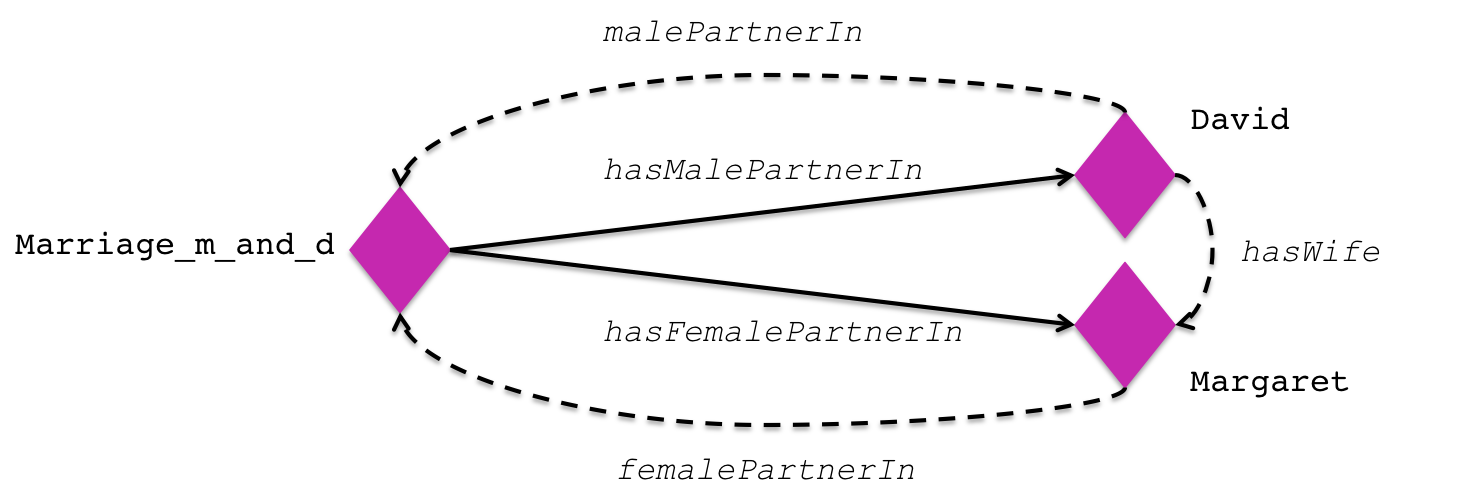
\includegraphics[width=\figwidth]{figures/spouse}
\caption{The sub-property chain path used to infer the spouse relationships via the marriage partnerships.}
\label{fig:spouse}
\end{center}
\end{figure}

The following questions can now be asked:
\begin{itemize}
\item Is wife of \ds;
\item Has a husband born before 1940;
\item The wife of an uncle of William Bright 1970. 
%\item \comment{some sensible task here}
\end{itemize}
\noindent and many more. This is really a chance to explore your querying abilities and make some complex nested queries  that involve going up and down the hierarchy and tracing routes through the  graph of relationships between the individuals you've inferred.

\section{In-Laws}

Now we have spouses, we can also have in-laws. The path is simple: \con{isSpouseOf o hasMother} implies \con{hasMotherInLaw}. The path involved in mother-in-laws can be seen in Figure~\ref{fig:mother-in-law}.
The following OWL code establishes the sub-property chains for \con{hasMotherInLaw}:
\\\\
\owlcode{
ObjectProperty: hasMotherInLaw

    SubPropertyOf:
        hasParentInLaw

    SubPropertyChain:
        isSpouseOf o hasMother

    Domain:
        Person

    Range:
        Woman

    InverseOf:
        isMotherInLawOf
}
\\
\begin{figure}
\begin{center}
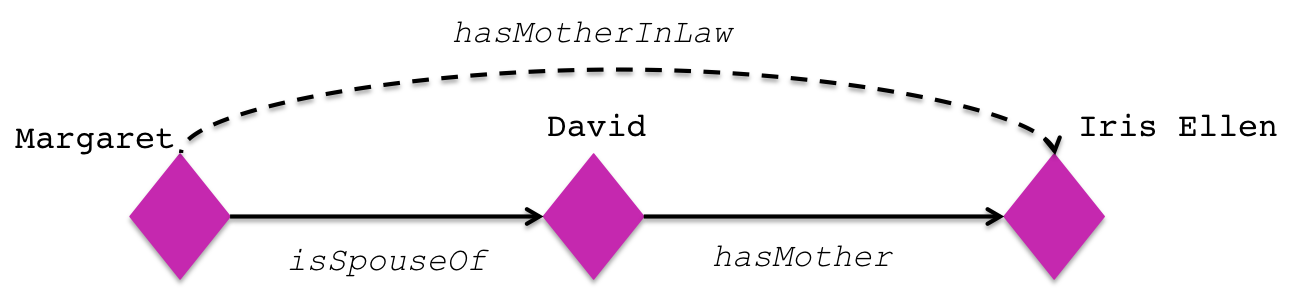
\includegraphics[width=\figwidth]{figures/mother_in_law}
\caption{Tracing out the path between objects to make the sub-property chain for mother-inlaws}
\label{fig:mother-in-law}
\end{center}
\end{figure}

Do the following to make the parent in-law properties:
\steps{Parents in-law}{
\item Create \con{hasParentInLaw} with two sub-properties of \con{hasMotherInLaw} and \con{hasFatherInLaw};
\item Create the inverses, but remember to let the reasoner infer the hierarchy on that side of the hierarchy;
\item Add the sub-property chains as described in the pattern for \con{hasMotherInLaw} above;
\item Run the reasoner and check that the mother-in-law of \mgs is Iris Ellen Archer.
}

\section{Brothers and Sisters In-Law}

Brothers and sisters in law have the interesting addition of having more than one path between objects to establish a sister or brother in law relationship. The OWL code below establishes the relationships for `is sister in law of':
\\\\
\owlcode{
ObjectProperty: hasSisterInLaw

    SubPropertyOf:
        hasSiblingInLaw

    SubPropertyChain:
        hasSpouse o hasSister

    SubPropertyChain:
        hasSibling o isWifeOf
}
\\
A wife's husband's sister is a sister in law of the wife. Figure~\ref{fig:sister-in-law} shows the two routes to being a sister-in-law. In addition, the wife is a sister in law of the husband's siblings. One can add as many sub-property chains to a property as one needs. You should add the properties for \con{hasSiblingInLawOf} and its obvious sub-properties following the inverse of the pattern above.

\steps{Siblings in-law}{
\item Create the relationships for siblings-in-law as indicated in the owl code above.
%\comment{explanation?}.
}
\dragon{By now, chances are high that the realisation takes a long time. We recommend to remove the very computationally expensive restriction \con{hasParent exactly 2 Person} on the \person class, if you have not done it so far.}

\begin{figure}
\begin{center}
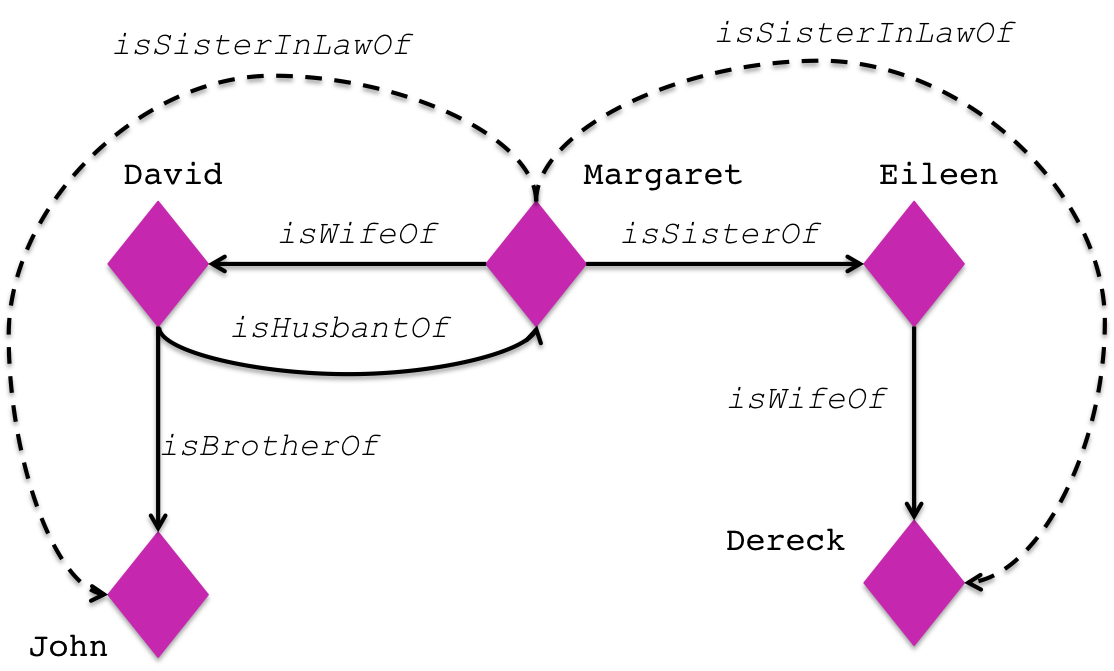
\includegraphics[width=\figwidth]{figures/sister_in_law}
\caption{The two routes to being a sister-in-law.}
\label{fig:sister-in-law}
\end{center}
\end{figure}

\section{Aunts and Uncles in-Law}
\label{sec:uncle-in-law}

The uncle of \rds has a wife, but she is not the aunt of \rds, she is the aunt-in-law. This is another kith relationship, not a kin relationship. The pattern has a familiar feel:
\\\\
\owlcode{
ObjectProperty: isAuntInLawOf

    SubPropertyOf:
        isInLawOf

    SubPropertyChain:
        isWifeOf o isBrotherOf o isParentOf
}
\\
\steps{Uncles and aunts in-law}{
\item Create \con{hasAuntInLaw} and \con{hasUncleInLaw} in the usual way;
\item Test in the usual way;
\item Tidy up the top of the property hierarchy so that it looks like Figure~\ref{fig:prop_marriage}. We have a top property of \con{hasRelation} and two sub-properties of \con{isBloodRelationOf} and \con{isInLawOf} to establish the kith and kin relationships respectively;
\item All the properties created in this chapter (except for spouses) should be underneath \con{isInLawOf}.
}

\begin{figure}
\begin{center}
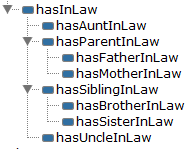
\includegraphics[width=\figwidth]{figures/new/prophierarchyinlaw}
\caption{The object property hierarchy after adding the various in-law properties.}
\label{fig:prop_marriage}
\end{center}
\end{figure}

\section{Summary}
This has really been a revision chapter; nothing new has really been introduced. We have added a lot of new object properties and one new data property. The latest object property hierarchy with the `in-law' branch can be seen in Figure~\ref{fig:prop_marriage}. Highlights have been:

\begin{itemize}
\item Having an explicit marriage object so that we can say things about the marriage itself, not just the people in the marriage;
\item We have seen that more than one property chain can be added to a property;
\item We have added a lot of kith relationships to join the kin or blood relationships;
\item As usual, the reasoner can establish the hierarchy for the inverses and put a lot of the domain and ranges in for free.
\end{itemize}

\expressivity{SROIQ(D)}

\ctime{0}{123655}{1618}